\begin{frame}{Pragmatism}
    \begin{columns}[c]
        \column{0.8\columnwidth}
        \begin{itemize}
            \item Many views, we'll \emph{mostly} focus on one:
            \begin{cquote}
                Knowledge is any rule or practice that ``works''.
            \end{cquote}
            \item Basically, we'll consider some rule or pattern \bhighlight{true} if the predictions we make according to it turn out correct.
            \item Known as \bhighlight{Pragmatism}.
        \end{itemize}
        \column{0.2\columnwidth}
        \begin{figure}
                \centering
                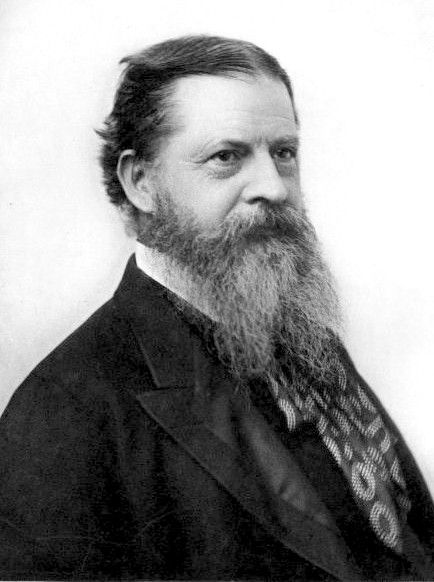
\includegraphics[width=\columnwidth]{images/Charles_Sanders_Peirce.jpg} % replace with your image file
                \caption{Charles Sanders Peirce --- mathematician and philosopher, and considered to be the father of Pragmatism. \gcite{\href{https://en.wikipedia.org/wiki/File:Charles_Sanders_Peirce.jpg}{Source}}}
            \end{figure}
    \end{columns}
\end{frame}

% \begin{frame}{Pragmatism}
%     \begin{columns}[c]
%         \begin{column}{0.80\textwidth}
%             \vfill
%             \begin{quote}
%                 ``All models are wrong, but some are useful." --- George Box
%             \end{quote}
%             \vfill
%         \end{column}
%         \begin{column}{0.20\textwidth}
%             \begin{figure}
%                 \centering
%                 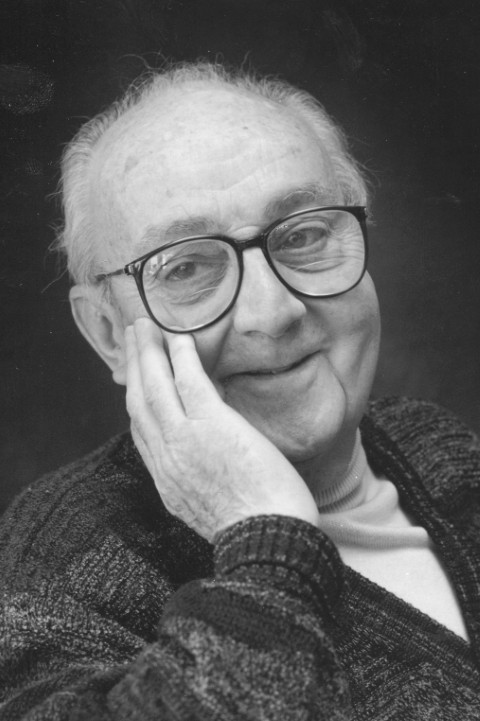
\includegraphics[width=\columnwidth]{images/george-ep-box.jpg} % replace with your image file
%                 \caption{George E.P. Box --- One of the great statistians of the 20th century. \gcite{\href{https://commons.wikimedia.org/w/index.php?curid=115167166}{Source}}}
%             \end{figure}
%         \end{column}
%     \end{columns}
% \end{frame}

% \begin{frame}{The pragmatic cycle}
%     \begin{figure}
%         \centering
%         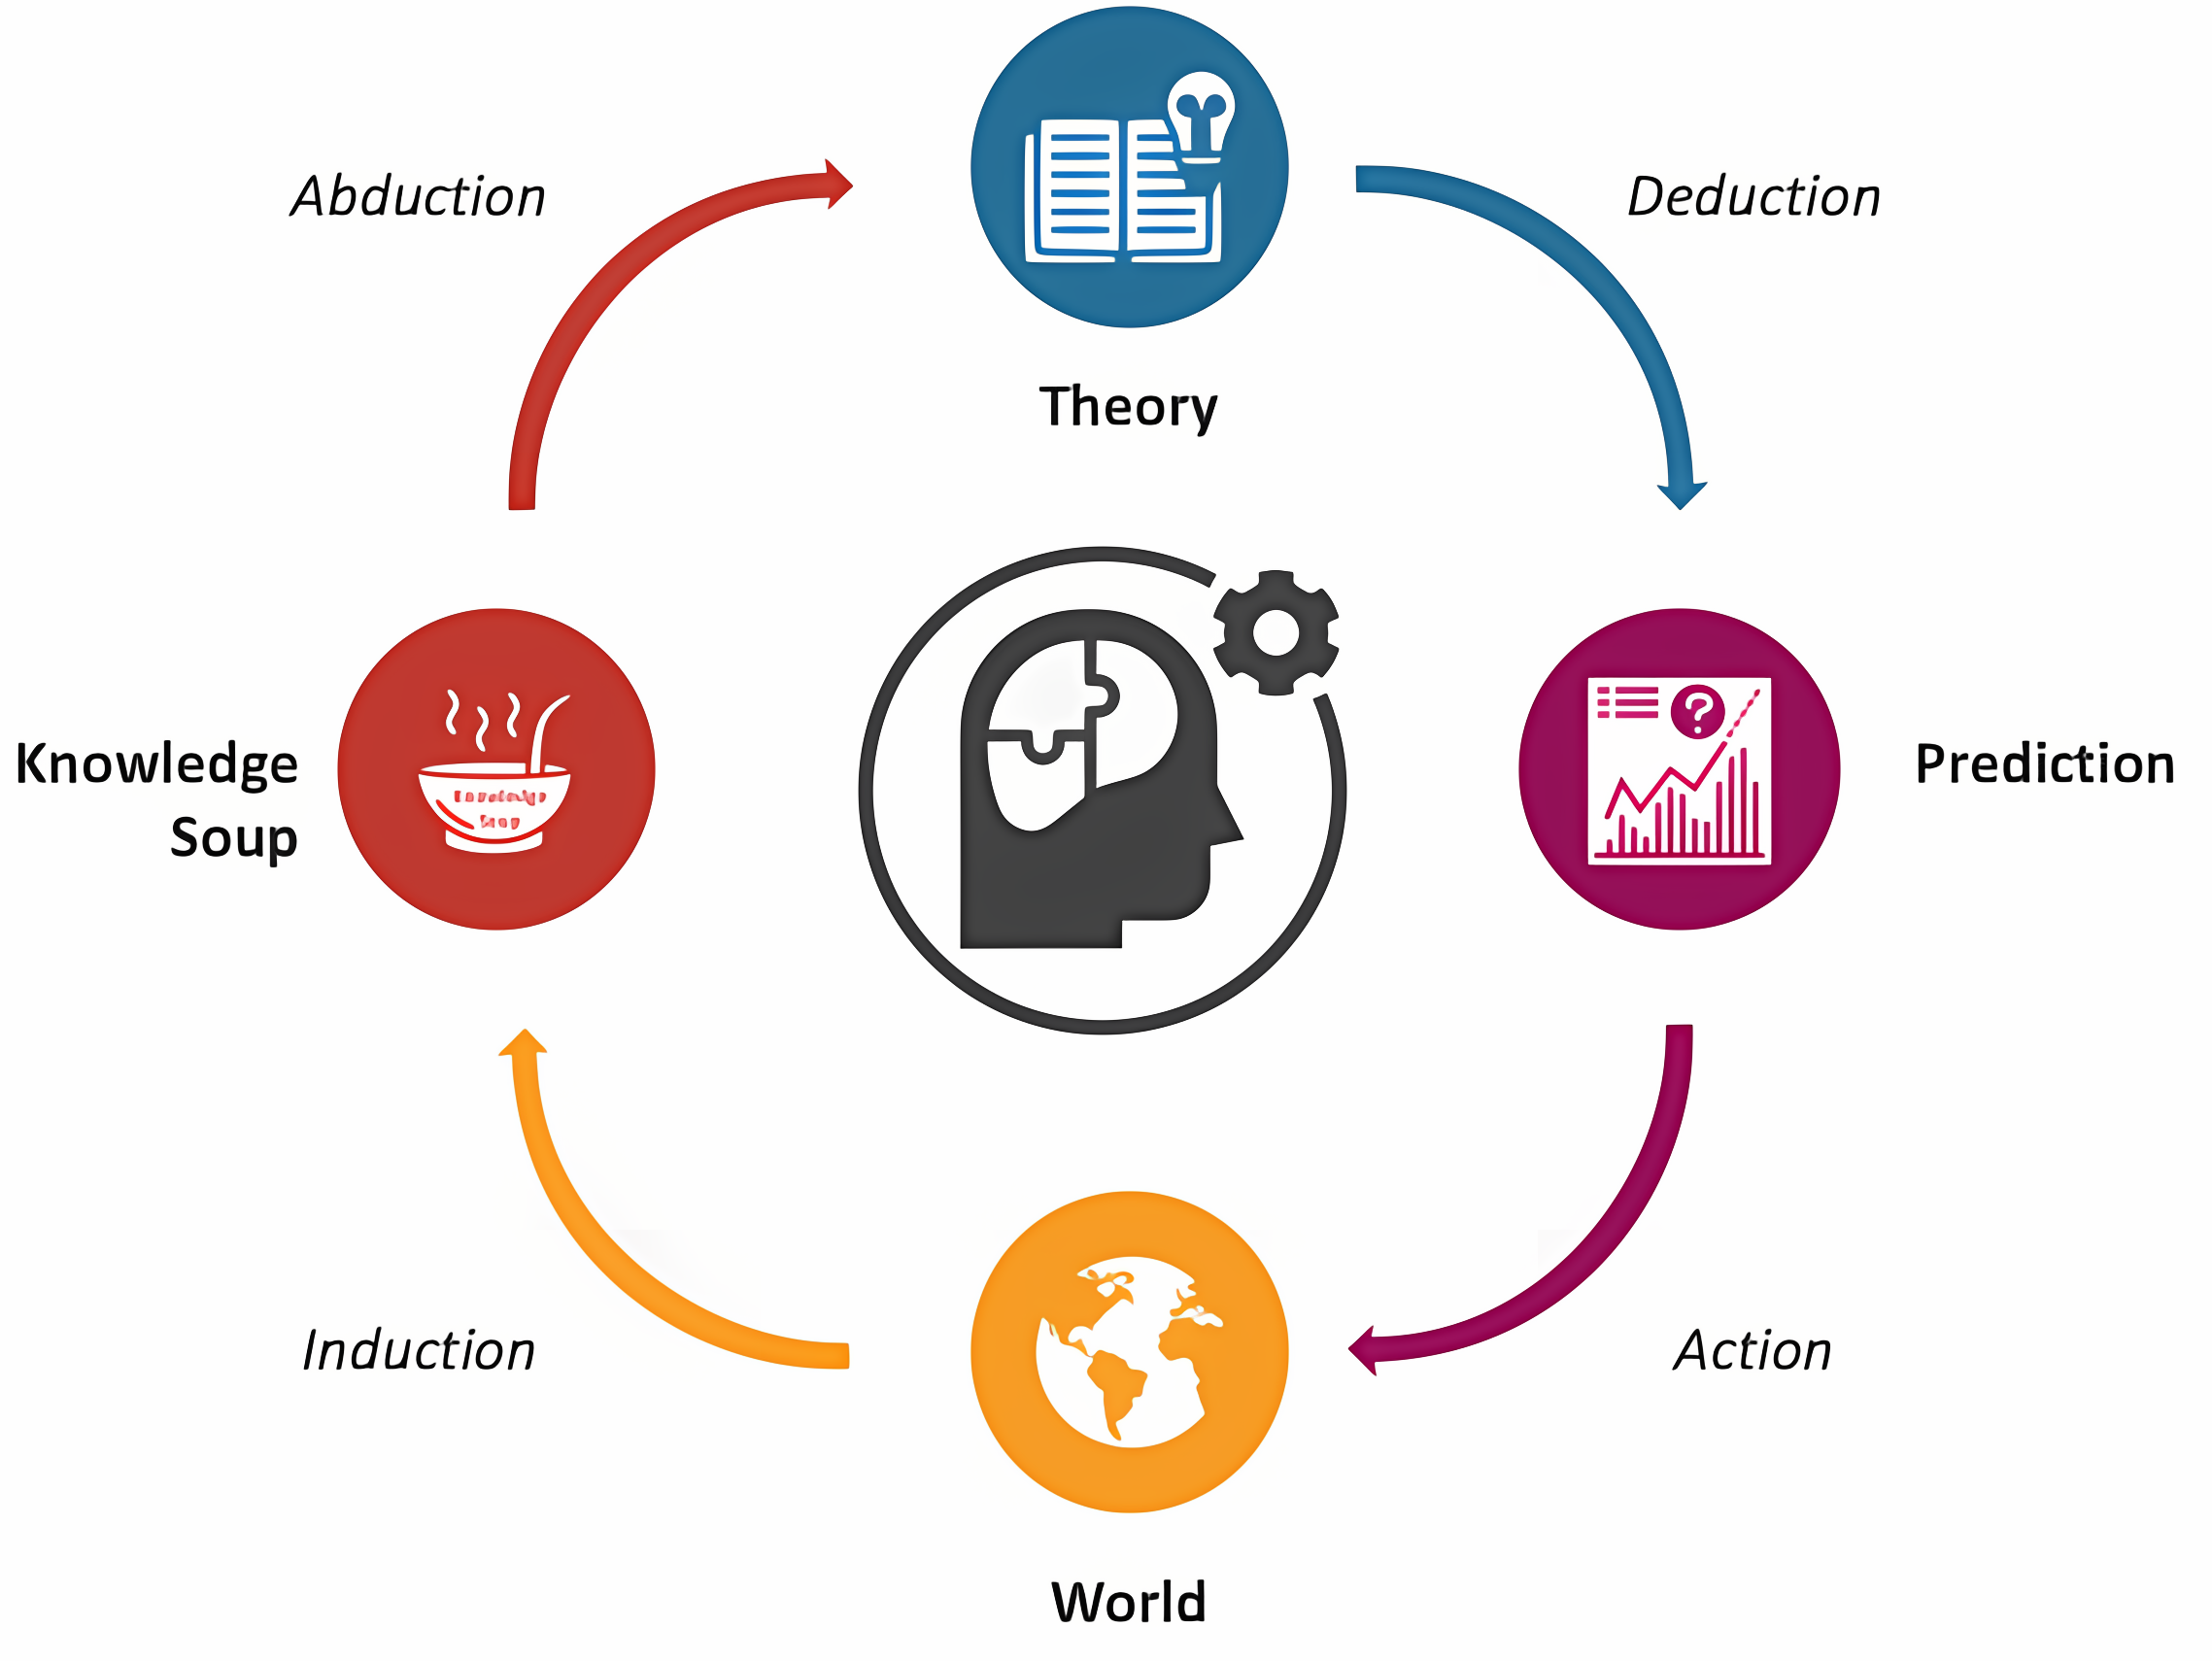
\includegraphics[width=0.8\textwidth]{images/pragmatism.png}
%         \caption{Peirce's cycle of Pragmatism. \gcite{\href{https://www.collidu.com/presentation-pragmatism}{Source}}}
%     \end{figure}
% \end{frame}